\par The classification problem introduces the concept of labels. They are discrete values, usually numerical, that are predicted by a function $f:D\rightarrow L$, where $D$ is the input domain, and $L$ is a finite set of labels. However, this mathematical approach makes it struggling to optimize the objective function, due to the fact that $L$ is not a continuous set, so $f$ cannot be differentiable. We might want to assure the continuity of $f$. Even though various solution may be propose to this problem, like interpolating between the label values (like ${0,1}$ or ${-1,1}$ for binary classification), we will focus on the probabilistic approach of letting $L=\{ l | l=(l_1,\ldots,l_n)\in\mathbb{R}^{n}, l_1+\ldots+l_n=1, l_i\geq 0\}$ be a vector set whose components at position $i$ are interpreted as the probability of the input data to be of label $i$ \cite{D2l}. For $n=2$, we are faced with a binary classification problem. A multi-class classification can be reduced to a binary classification problem by choosing the output form to be a list of $\mathbb{R}^2$ categorical vectors, each one representing a confidence factor of a certain label to be a true class of the analyzed data. This last model is also suitable for multi-label classification, the type of problem where an input can belong to one or more classes \cite{D2l}.
\par The last step in such a classification approach is collapsing the continuous output to a discrete label value. As we have observed, for a probabilistic model the discrete output would be the index of the label that appears with the highest probability. In case of a general continuous model, some threshold would apply to obtain the closest integer label according to problem-specific chosen conditions.


\subsubsection{Classification losses}
\label{subsubsec:ch3sec2subsec4subsubsec1}

\par In other words, classification problems can be therefore transformed into regression problems by relaxing the output constraints. Intuitively, instead of requiring the predicted value $\mathrm{y}^\star$ to be either a fixed $0$ or $1$, we can allow the function to predict continuous values based on which one could eventually make a final decision regarding the predicted class. A simple example of reasoning would be to consider that $\mathrm{x}$ for which $\mathrm{y}^\star=f(\mathrm{x}) \geq 0.5$ are more likely to have their corresponding output $\mathrm{y}=1$ than of class $\mathrm{y}=0$. Such $y^\star$ are called logits. Furthermore, this "likeliness" idea conduces to a more formal description that can be also generalized to multi-label classification. Our function will try to predict a vector of probabilities of the same length as the number of classes where the probabilities add up to 1 \cite{losssurvey}. The prediction function is trying to raise the probability of the real labels while lowering the potential for a mistaken guess. A remarkable type of classification loss is the cross entropy loss that takes advantage of the properties of probabilities distributions: $\textit{crossentropy}(\mathrm{y}, \mathrm{y^\star}) = -\sum_{i=0}^n{\mathrm{y_i} \log{\mathrm{y_i^\star}}}$ \cite{losssurvey}.

\begin{table}[htbp]
\begin{center}
\begin{tabular}
{|p{120pt}|p{120pt}|p{120pt}|}
\hline
 Name  &  Formula & Usage\\
\hline Hinge loss & $\max(0, 1-\mathrm{y}^\star \mathrm{y})$ & for ${-1,1}$ outputs \\
\hline Cosine similarity & $1-\mathrm{y}^\star \mathrm{y} / (||\mathrm{y}|| \cdot ||\mathrm{y}^\star||)$ & when direction matters more than magnitude\\

\hline Kullback-Leibler divergence  & $\sum_{i}{\mathrm{y_i} (\log{\mathrm{y_i}} - \log{\mathrm{y_i^\star}})}$ & applications in GANs\\
\hline
\end{tabular}
\end{center}
\caption{Other classification losses \cite{losssurvey} }
\label{ClassLosses}
\end{table}

\subsubsection{Softmax}
\label{subsubsec:ch3sec2subsec4subsubsec2}

One of the first challenges of classification is to ensure that the prediction output is in the bounds of the defined model. We do not allow number that describe probabilities to be out of the interval $[0,1]$. Furthermore, in the case of categorical data, we must make sure the sum of probabilities is equal to $1$. The softmax \cite{softmax} as an activation function solves all the mentioned problems:
$$\mathrm{softmax}(x)=\left(\frac{e^{x_i}}{\sum_{j=1}^n{e^{x_j}}}\right)_{i=\overline{1,n}}.$$
While it acts as a normalizer on the function's output, this function keeps the order of confidence indicators. We can extract the predicted label by performing an $\mathrm{argmax}$ operation on the output of $\mathrm{softmax}$. Some approaches \cite{softargmax} even propose a soft-argmax function,
$$\mathrm{softargmax}(x)=\sum_{i=1}^n\frac{e^{\beta x_i}}{\sum_{j=1}^n{e^{\beta x_j}}} i, \beta\in\mathbb{R}$$
By choosing $\beta$ large enough, the dominant feature will become even more intense, up to the point where its probability would almost reach $1$, while the others represent only a tiny fraction of the whole, thus the most significant weight is given to a label $k$ that would be easily reconstructible from the output of softargmax by simple rounding to the closest integer. The exponential here may helps accelerate the growth and distinguish between close probabilities by creating a magnitude level difference between them. Thus we have a differentiable function that also directly predicts labels indices. By choosing $b=\frac{1}{T}$, the formula above becomes the softmax with temperature loss, $\frac{\exp{(x_i/T)}}{\sum_{j=1}^ n{\exp{(x_j/T)}}}$. High values of the temperature $T$ result in increases the smoothness of the problability distribution, while lower values of $T$ encourage randomness. Making $T=1$ lets the distribution unchanged \cite{hinton2015distilling}. The temperature softmax has seen practical use in Large Language Models (LLMs) when it comes to adjusting the level of creativity or repetition in the generated text output of the model \cite{renze2024effect}.
%\marginpar{\textcolor{green}{eu as aminti si de versiunea de softmax cu T (temperature) - cea folosita in LLM-uri si care are efecte asupra diversitatii outputurilor produse}}

\subsection{Performance metrics}
\label{subsubsec:ch3sec2subsec4subsubsec3}

As opposed to the regression problems, where an error is used to measure the performance of the model, classification problems allow for a more detailed metrics to report how well it behaved on the target data. These metrics have roots in the theory of statistics. One of them is the accuracy, which is defined as the fraction between the correctly predicted inputs and the total inputs count. For increased formality, let's recall the following definitions in the context of a true/false binary classification \cite{confmat}:
\begin{itemize}
\item True Positive (TP): a real positive value is correctly predicted as positive
\item False Positive (FP): a real negative value is wrongly predicted as positive
\item False Negative (FN): a real positive value is wrongly predicted as negative
\item True Negative (TN): a real negative value is correctly predicted as negative
\end{itemize} 
These are the building blocks the following classification metrics:
\begin{itemize}
\item Accuracy (measures the number of right predictions relative to the given data, it works best with balanced labeling) \cite{confmat}
$$\mathrm{accuracy} = \frac{TP+TN}{TP+TN+FP+FN}$$ 
\item Misclassification (measures the number of incorrect predictions) \cite{confmat}
$$\mathrm{misclassification} = \frac{FP+FN}{TP+TN+FP+FN} = 1-\mathrm{accuracy}$$ 
\item Precision (gives us the fraction of the correctly predicted values that were actually positive, it is a measure of reliability) \cite{confmat}
$$\mathrm{precision} = \frac{TP}{TP+TN}$$ 
\item Recall (the success rate of only predicting the positive values) \cite{confmat}
$$\mathrm{recall} = \frac{TP}{TP+FN}$$ 
\end{itemize}

\begin{figure}[htbp]
	\centering
	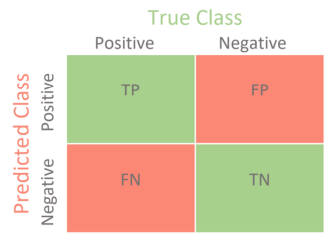
\includegraphics[scale=0.65]{figures/confmat.PNG}
	\caption{Confusion matrix for binary classification\cite{confmat}}
	\label{FigConfMatTF}
\end{figure}

The figure \ref{FigConfMatTF} displays the placement of the described values into a form of confusion matrix. For $n$-labels classification, a type of confusion matrix $C$ that takes into account not only the binary correctness state of prediction (if was right or not), but also the relations between each two labels $i$ and $j$ is illustrated in figure \ref{FigConfMatN}. Here, $C_{i j}$ represents the amount of ${i}$ labeled data that have been classified under label $j$. The metrics above can be generalized, globally or per each label, on this type of confusion matrix:
$$\mathrm{accuracy} = \frac{\sum_{i=1}^n{C_{i i}}}{\sum_{j=1}^n\sum_{i=1}^n{C_{i j}}}$$
$$\mathrm{precision}_i = \frac{C_{i i}}{\sum_{j=1}^n{C_{j i}}}$$
$$\mathrm{recall}_i = \frac{C_{i i}}{\sum_{j=1}^n{C_{i j}}}$$


\begin{figure}[htbp]
	\centering
	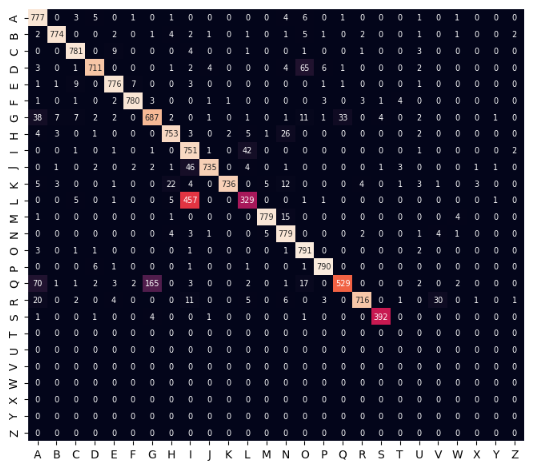
\includegraphics[scale=0.50]{figures/confmat_n.PNG}
	\caption{Confusion matrix for a custom trained EMNIST classification model}
	\label{FigConfMatN}
\end{figure}